In this explorative work, results will be shown for the how each
individual mesh operations (triangle split, edge split, node movement)
affects the representation deficit. In addition, an effective
combination of the aforementioned mesh operations was developed and the
results will be shown. The geometry which is being discretized is the
``peaks'' function which has a well-known parametrization
\cite{peaksMatlab}. The domain was chosen so that the boundary is
sufficiently far away from the local minima/maxima present near the origin to
show that the developed scheme is efficient at reducing representation
deficit. The $x$ and $y$ values are each confined between $-5.0$ and
$5.0$ and the initial triangulation is two triangles that fill the
quadrilateral defined by the four corner points.

The main driver of representation deficit, $RD$, based mesh refinement
is the value for representation deficit. This is a ratio of the
``before'' area to the ``after'' area for each mesh operation. The
surface area of the peaks function in the given domain was calculated by
uniformly triangulating the surface with a very fine resolution. The
result was found to converge to $177.944$ with a $u$ and $v$ resolution
of 301 points. For ease of presentation, the peaks functions is shown as
a contour plot where red represents local maxima and blue represents
local minima/maxima.

\subsection{Triangle and Edge Splitting}
Restricting the mesh refinement to only triangle splits or only edges
splits is not useful, as discussed above. Therefore, the combination of
the two was performed (as described in \ref{alg_IterativeRefinement})
to produce the following results. The following figure shows the results
from $tol_{RD}=\left(0.5,0.25,0.125\right)$ from left to right. The mesh was
refined by splitting triangles and edges where appropriate as described
above.

\begin{figure}[h!]
  \begin{center}
  \label{fig_RefineOnly}

  \subfloat[$tol_{RD}=0.5$]{\label{fig_RefineOnlyA}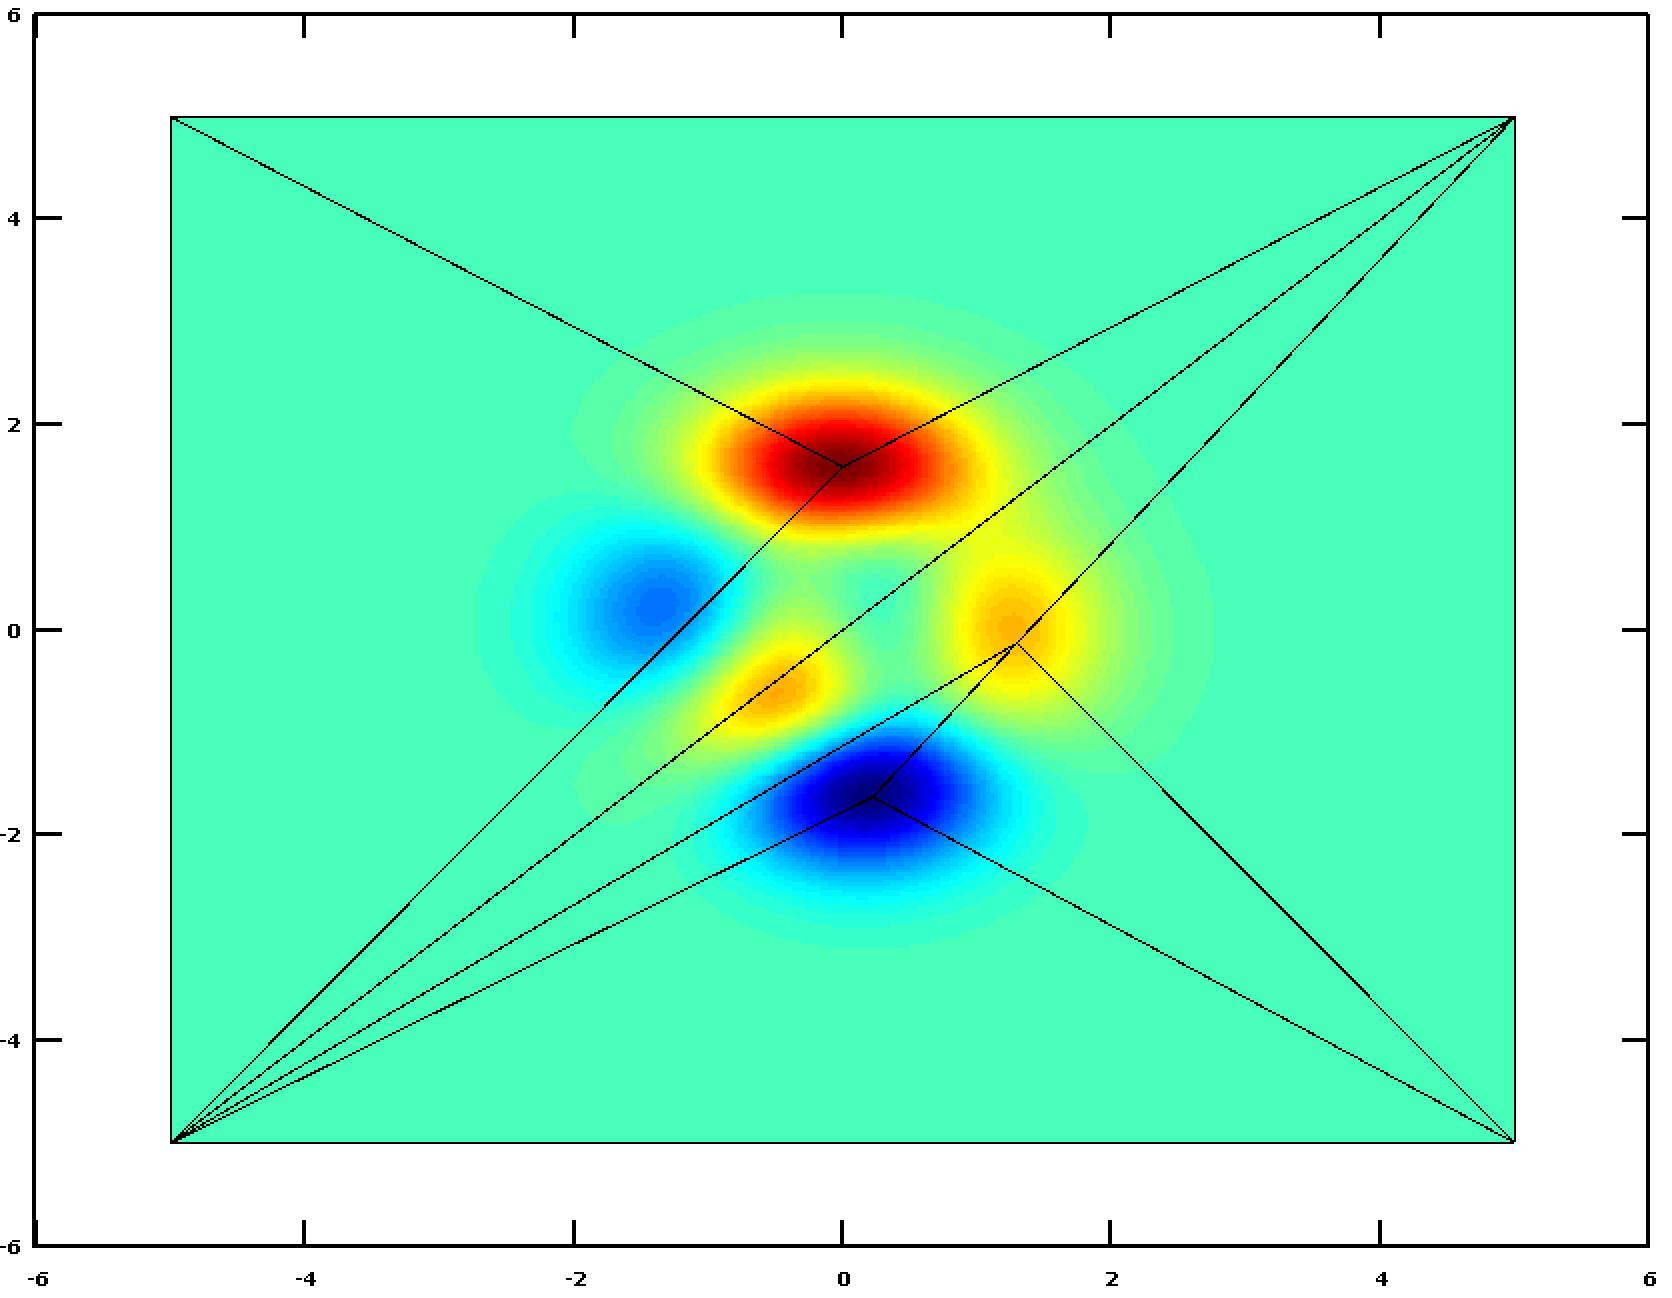
\includegraphics[width=50mm]{Figures/RefineOnly05.png}}
  \subfloat[$tol_{RD}=0.25$]{\label{fig_RefineOnlyB}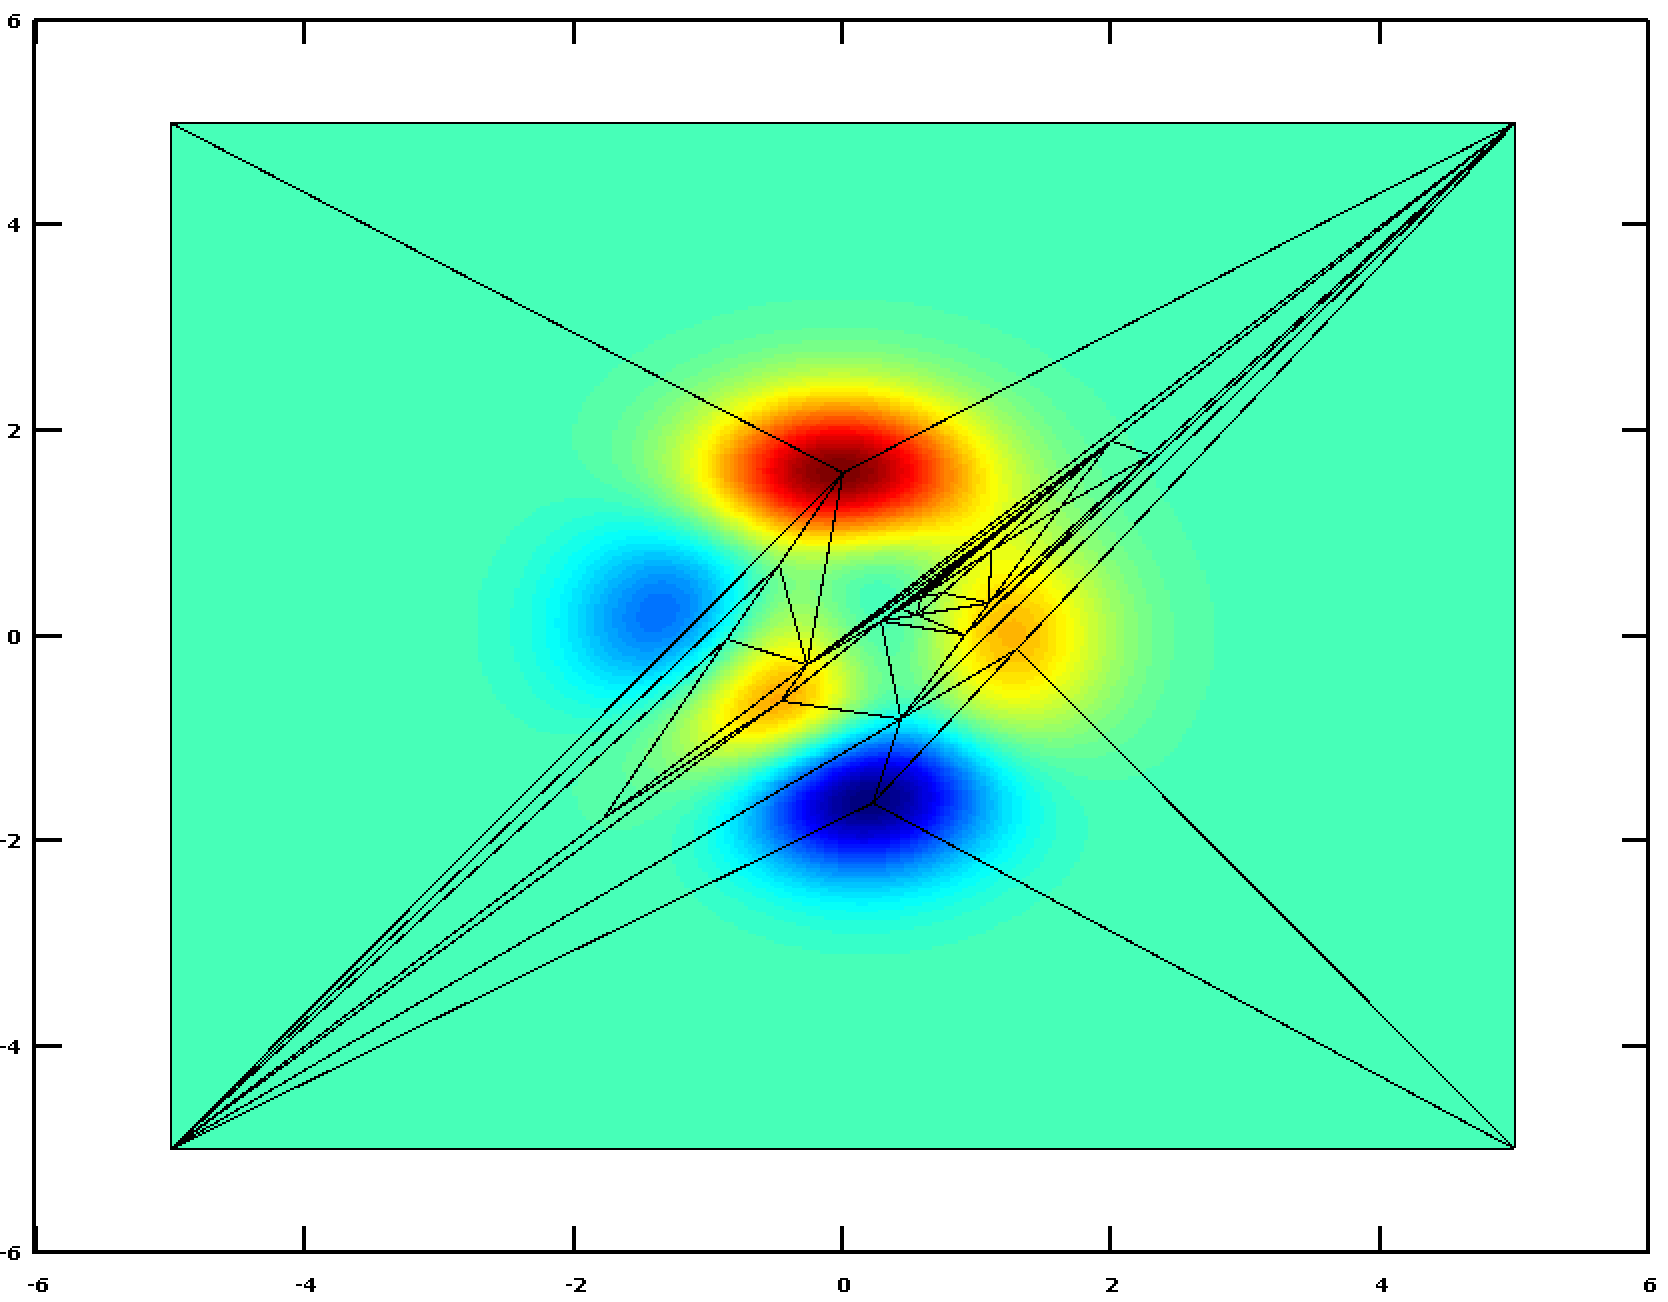
\includegraphics[width=50mm]{Figures/RefineOnly025.png}}
  \subfloat[$tol_{RD}=0.125$]{\label{fig_RefineOnlyC}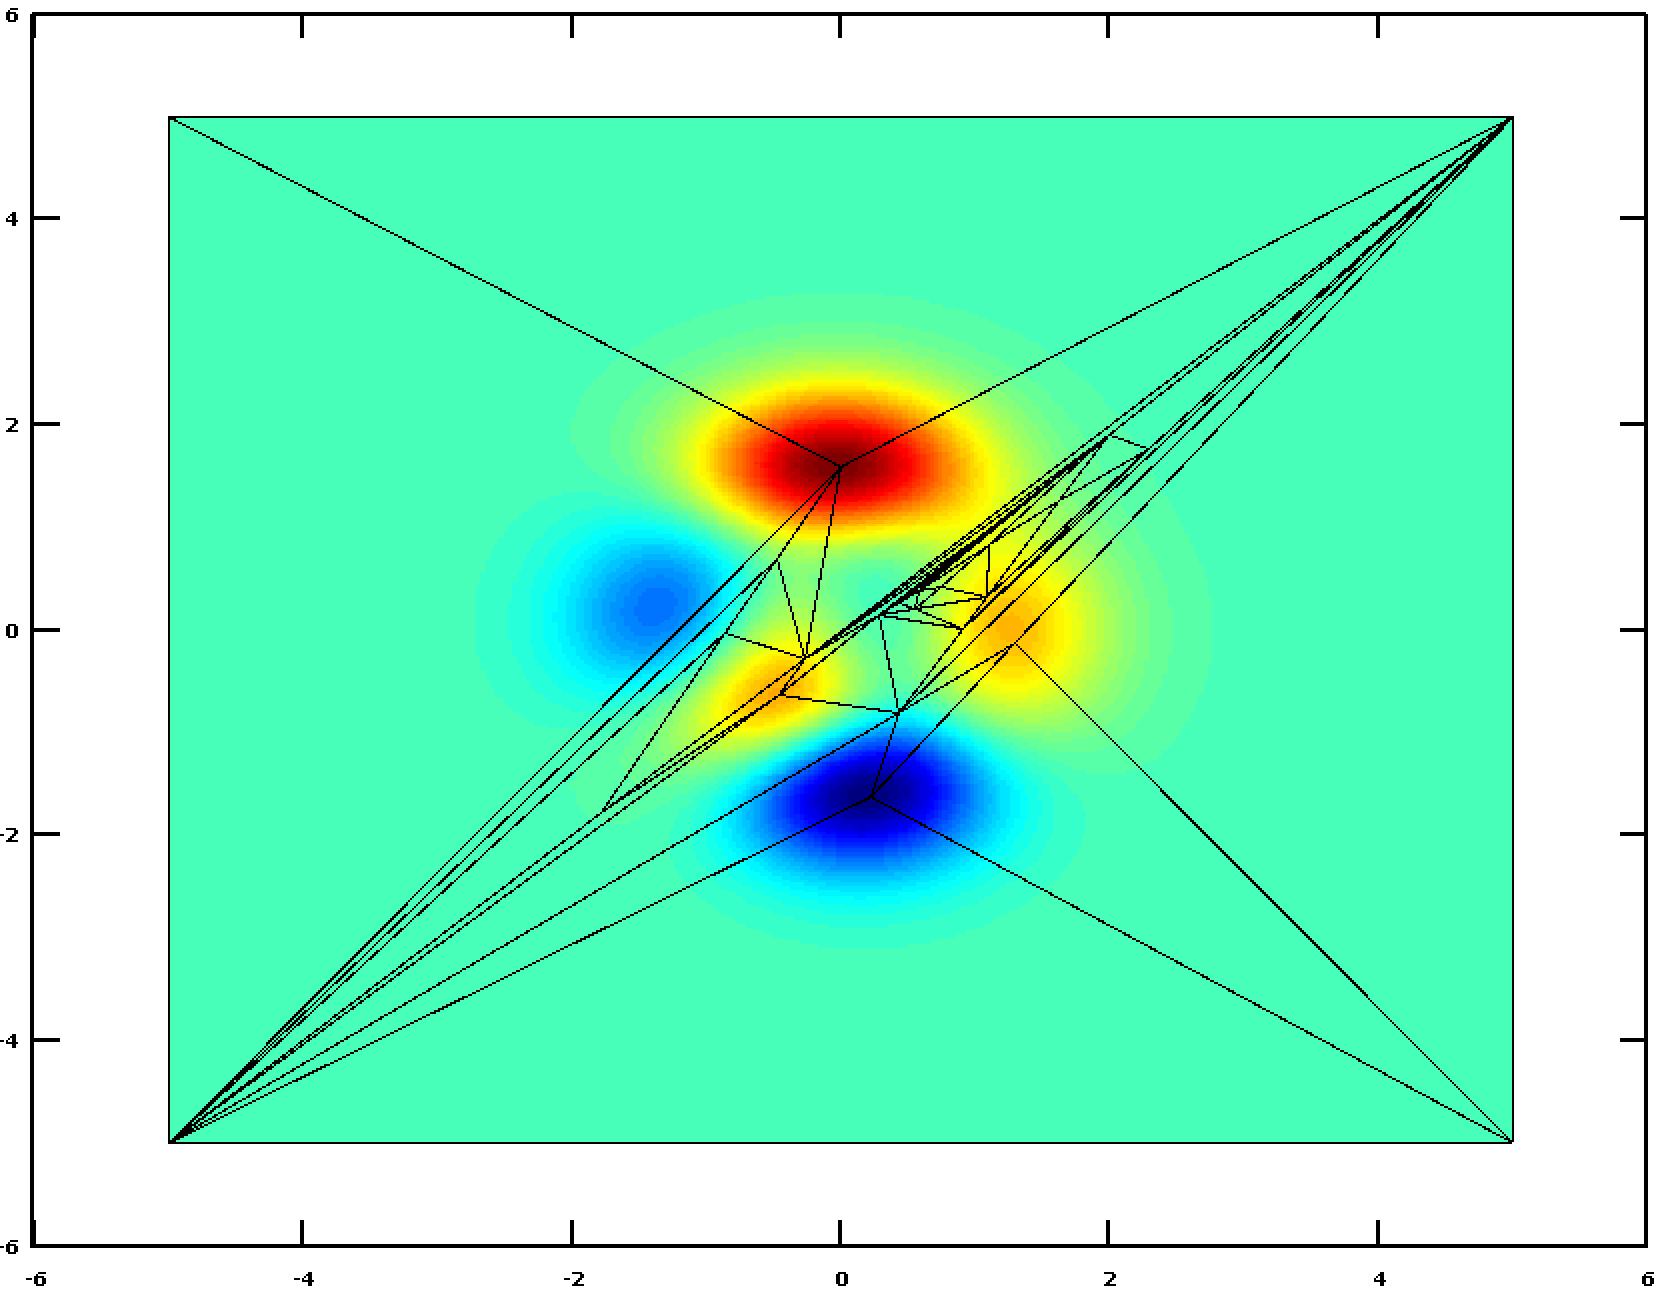
\includegraphics[width=50mm]{Figures/RefineOnly0125.png}}

  \caption{Mesh Refinement Only}
  \end{center}
\end{figure}

In \ref{fig_RefineOnlyA} it can be seen that only three nodes were
inserted. This is due to the very high value of $tol_{RD}$ for this
example.  However, the nodes that were inserted were inserted very near
to the local minima/maxima of the function. If $tol_{RD}$ were halved to
$0.25$, \ref{fig_RefineOnlyB} then $92$ nodes are inserted. Again, the
nodes are inserted very near to local minima/maxima and additionally
near saddle points. If $tol_{RD}$ is halved again to $0.125$,
\ref{fig_RefineOnlyC}, no more nodes are inserted. This is due to the
very poor quality triangles.  The sliver triangles that can be seen in
\ref{fig_RefineOnlyB}, \ref{fig_RefineOnlyC} represent nearly planar section
of the mesh and therefore not refined further. This is the major
shortcoming of the developed algorithm: element quality is not
considered and this limitation leads to poor quality meshes that cannot
be refined further.

\subsection{Node Movement Effect}
In order to show the effect of node movement, the resultant mesh shown
in \ref{fig_RefineOnlyB} is used as input and the same value for
$tol_{RD} = 0.25$ is used with \ref{alg_NodeSmoothing}.

\begin{figure}[h!]
  \begin{center}
  \label{fig_NodeSmoothing}
 
  \subfloat[$tol_{RD}=0.25$]{\label{fig_NodeSmoothingA}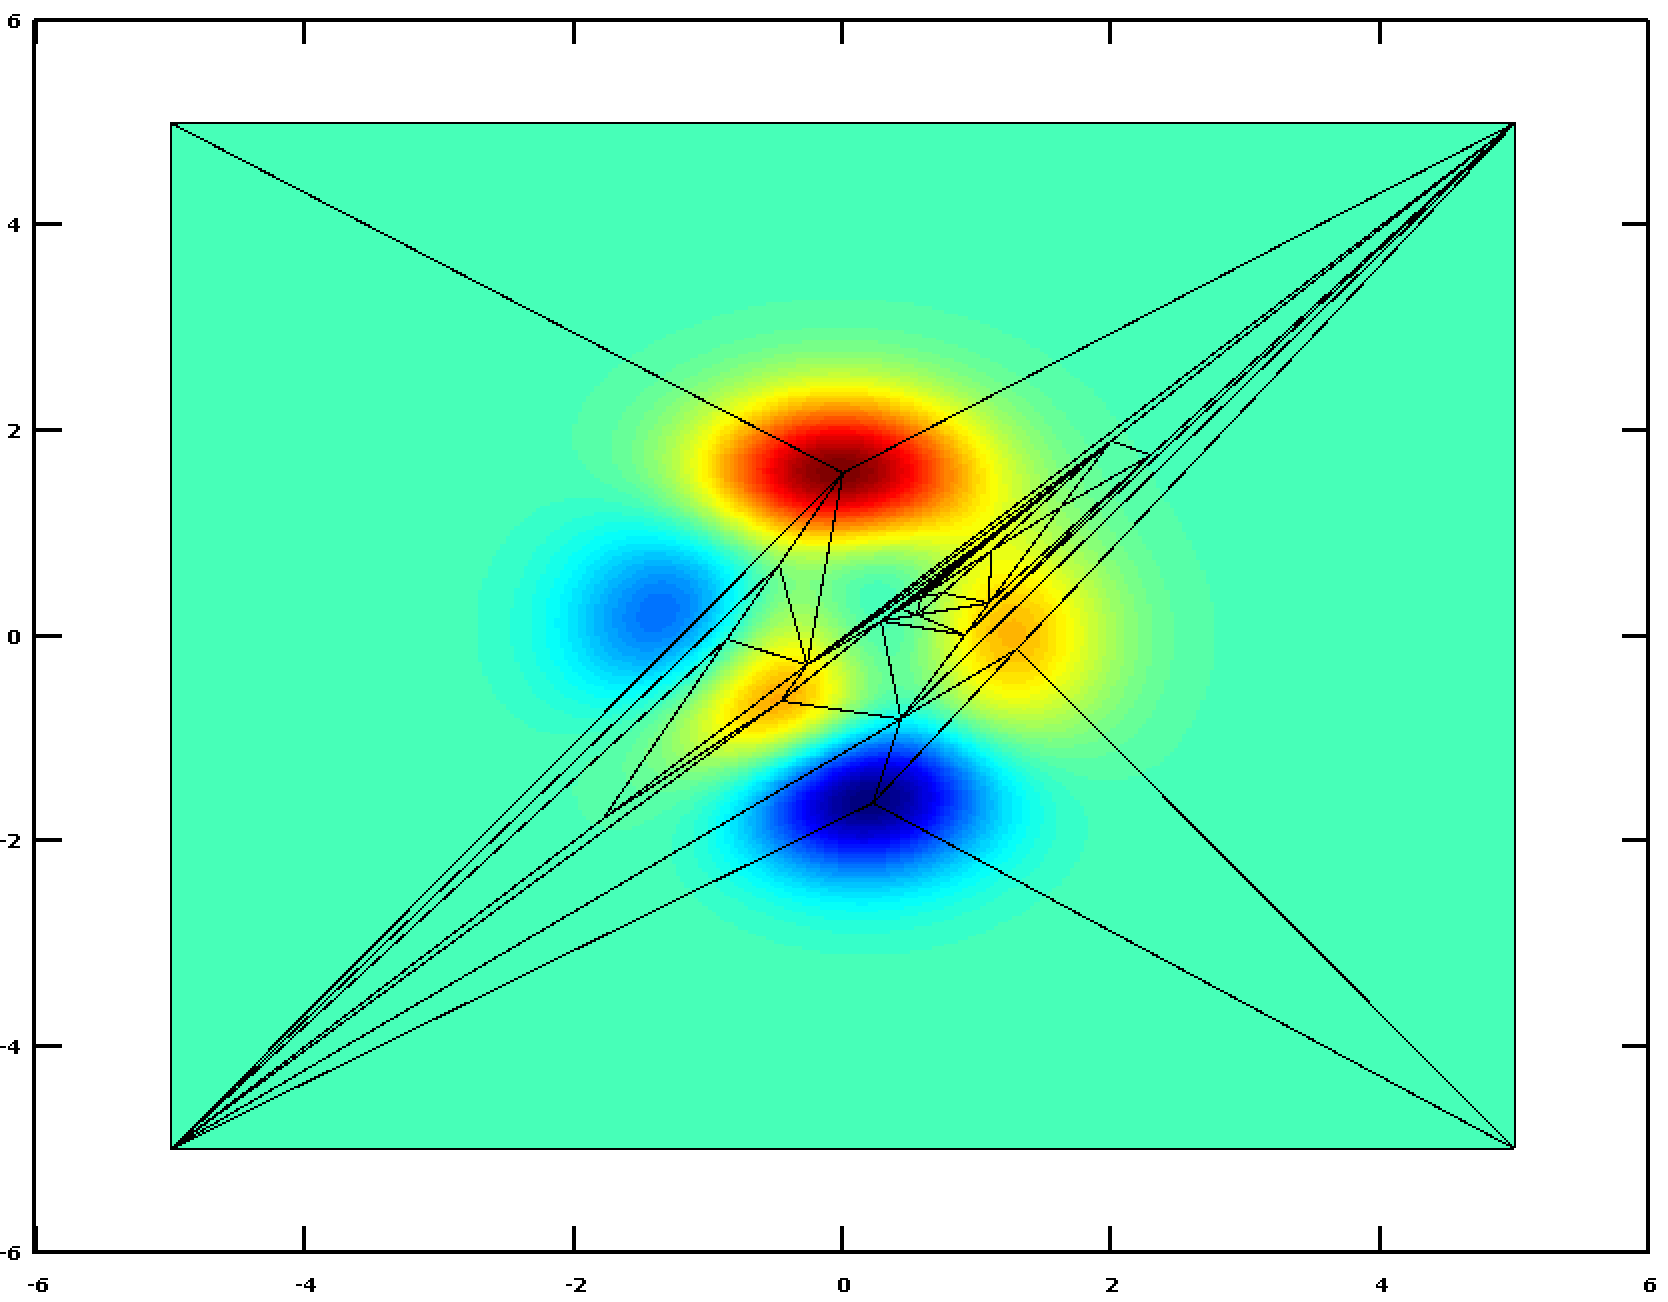
\includegraphics[width=60mm]{Figures/RefineOnly025.png}}
  \subfloat[$tol_{RD}=0.25$]{\label{fig_NodeSmoothingB}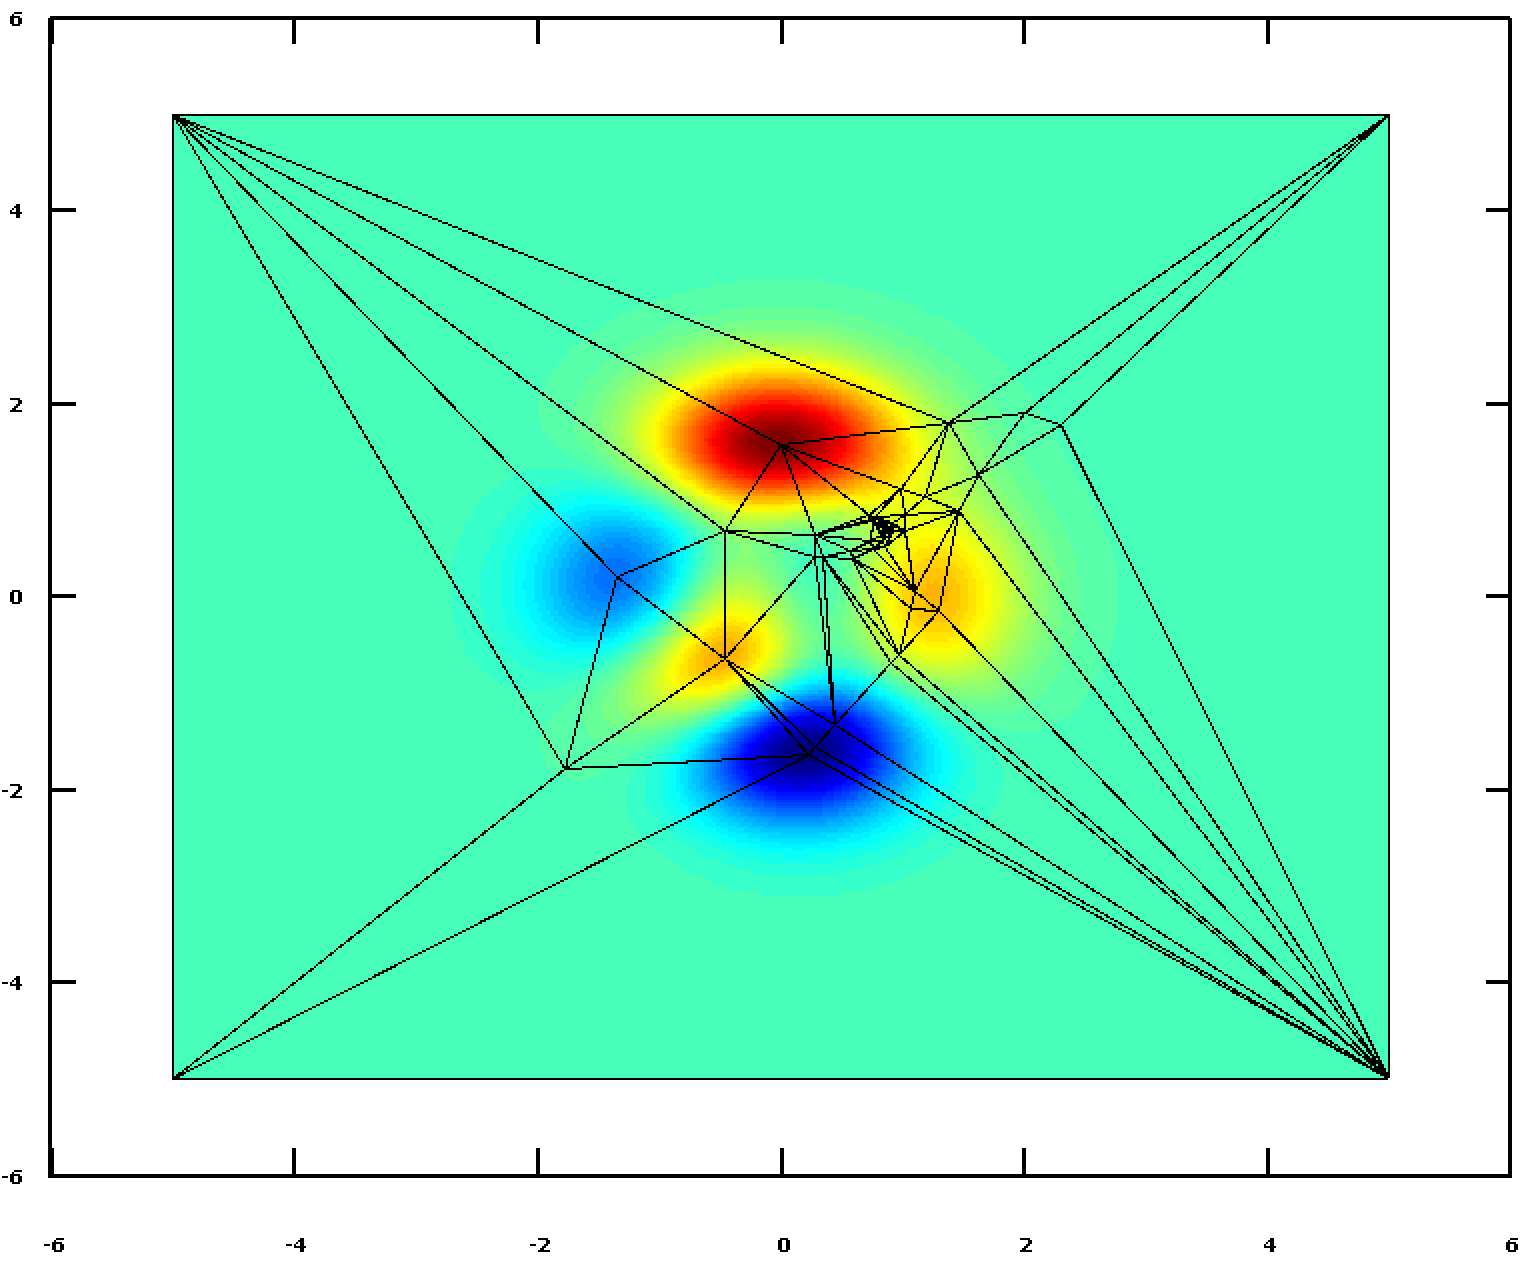
\includegraphics[width=60mm]{Figures/NodeSmooth025.png}}

  \end{center}
\end{figure}

The node movement was very effective at reducing representation deficit.
For this particular case, it reduced the representation deficit of the
input mesh by $23.36\%$. It should also be noted that the local
minima/maxima were accurately maintained by this procedure. It can also
be seen that moved nodes that were nearby but not in local minima/maxim
were moved to the local minima/maxima. Additionally, since the node
movement was allowed to perform local reconnections where needed
(discussed above), the element quality was also improved as a
side-effect.

\subsection{Effective Combination}
It easily noted that while the aforementioned mesh operations are
effective at reducing representation deficit they do not create high
quality triangles.  However, with the addition of a simple min-max edge
flip pass in between refinement and node movement passes the element
quality and representation deficit can be improved significantly.

\begin{figure}[h!]
  \begin{center}
  \label{fig_NodeSmoothing}
 
  \subfloat[$tol_{RD}=0.25$, no movement]{\label{fig_ComboA}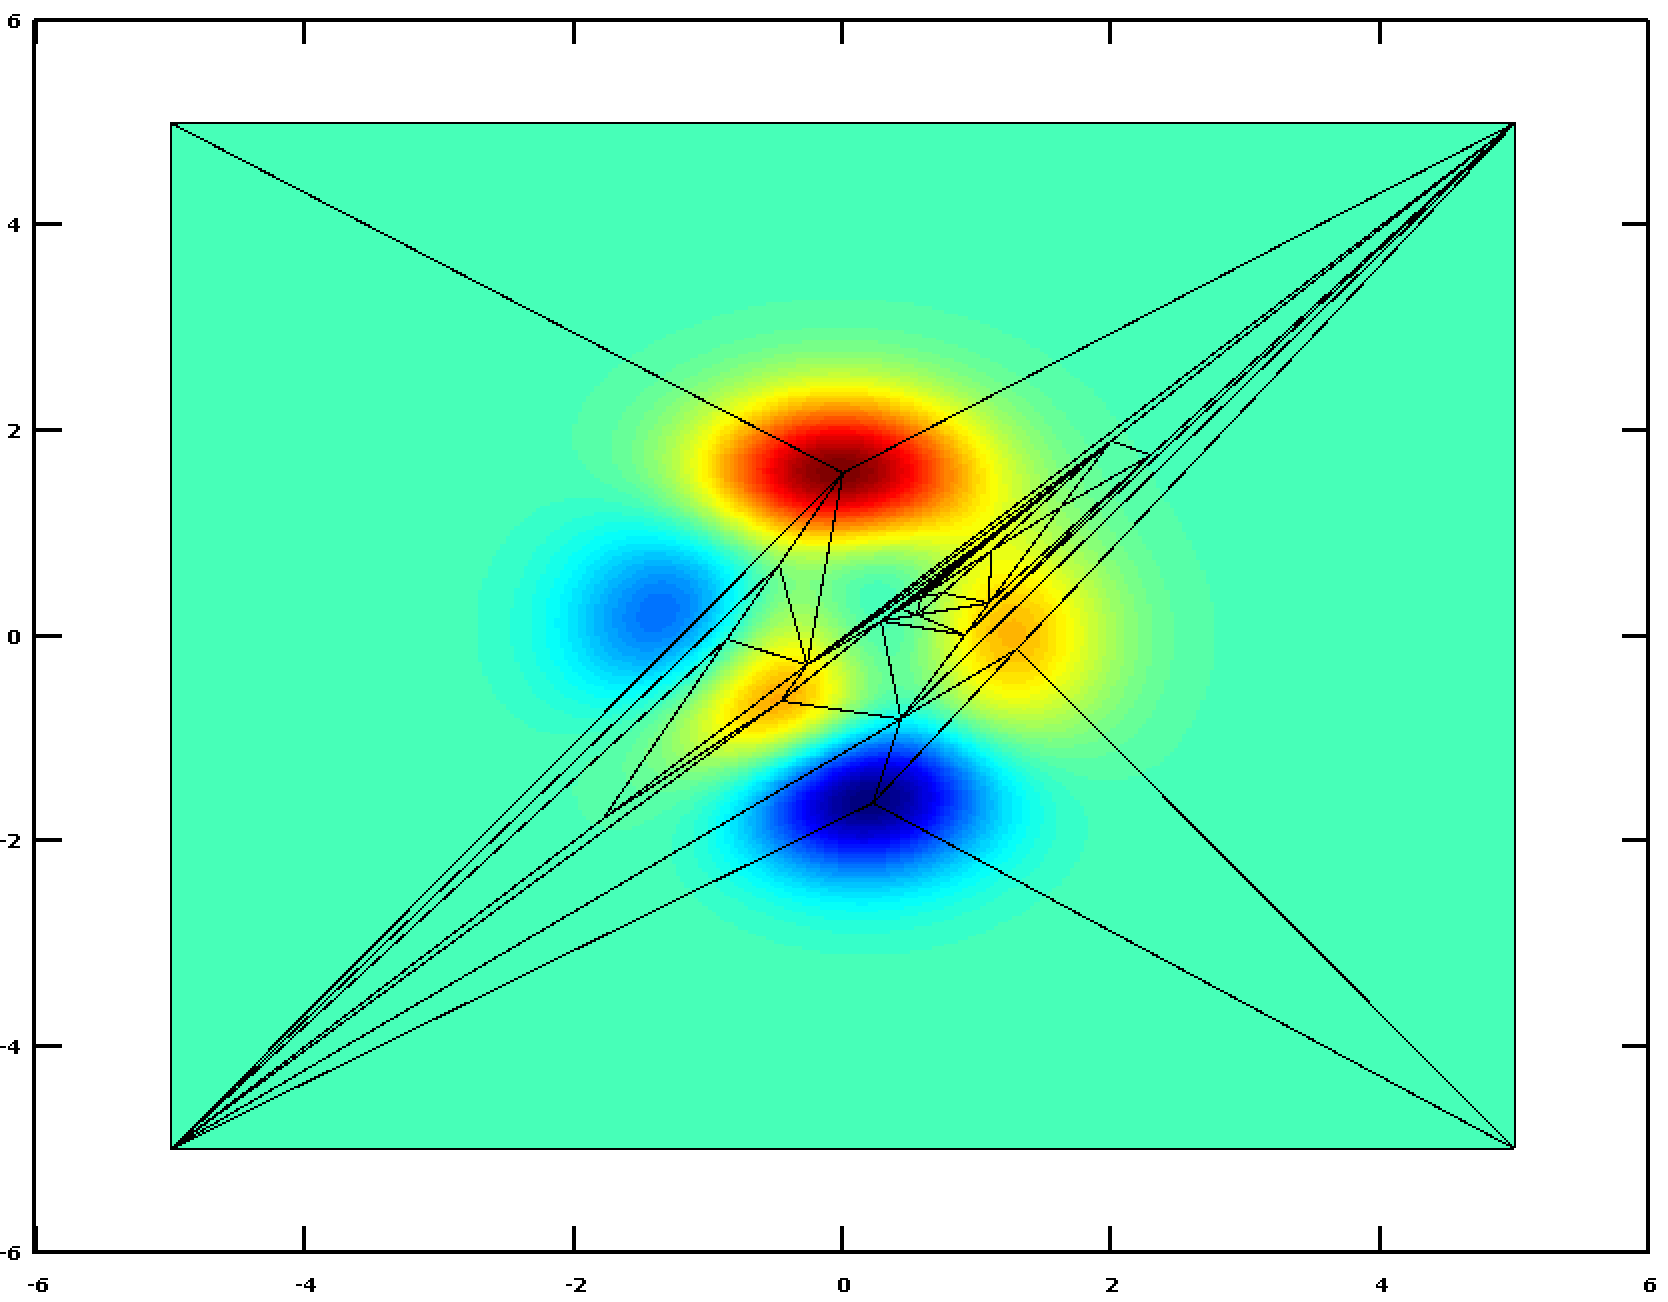
\includegraphics[width=50mm]{Figures/RefineOnly025.png}}
  \subfloat[$tol_{RD}=0.25$, movement post]{\label{fig_ComboB}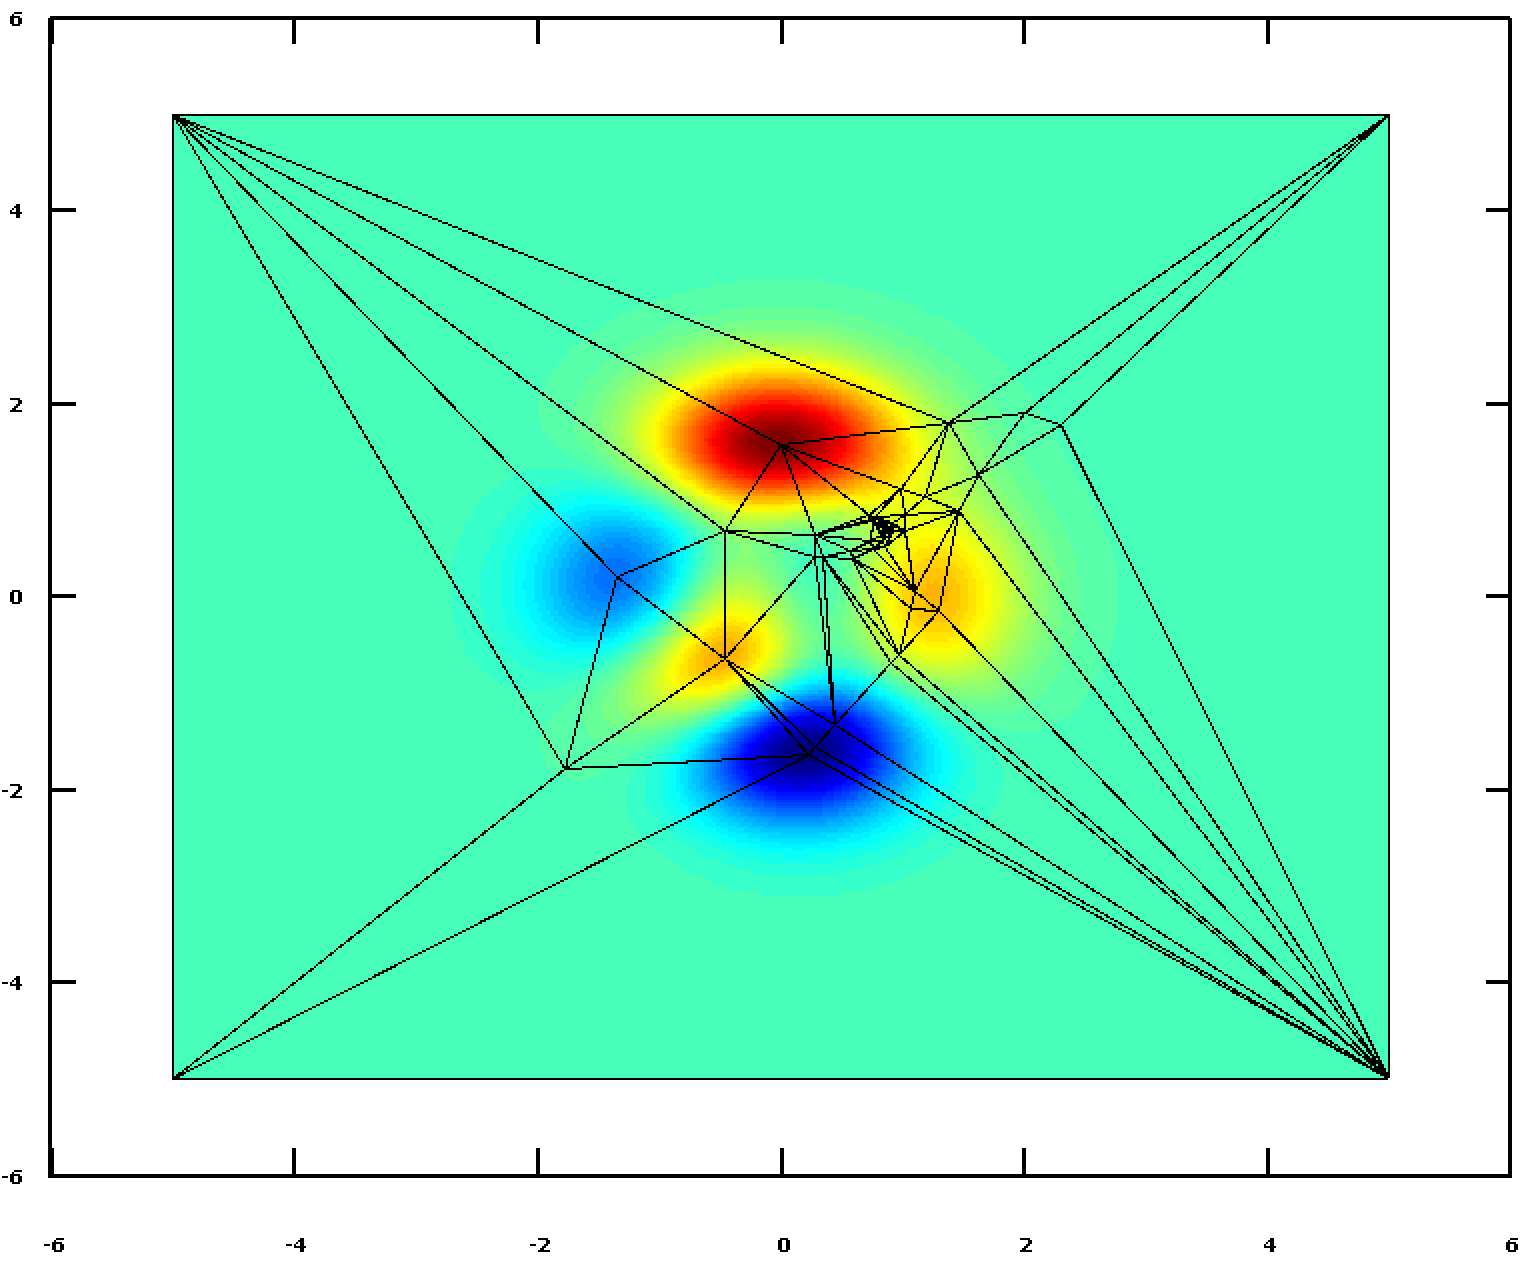
\includegraphics[width=50mm]{Figures/NodeSmooth025.png}}
  \subfloat[$tol_{RD}=0.25$, reconnection]{\label{fig_ComboC}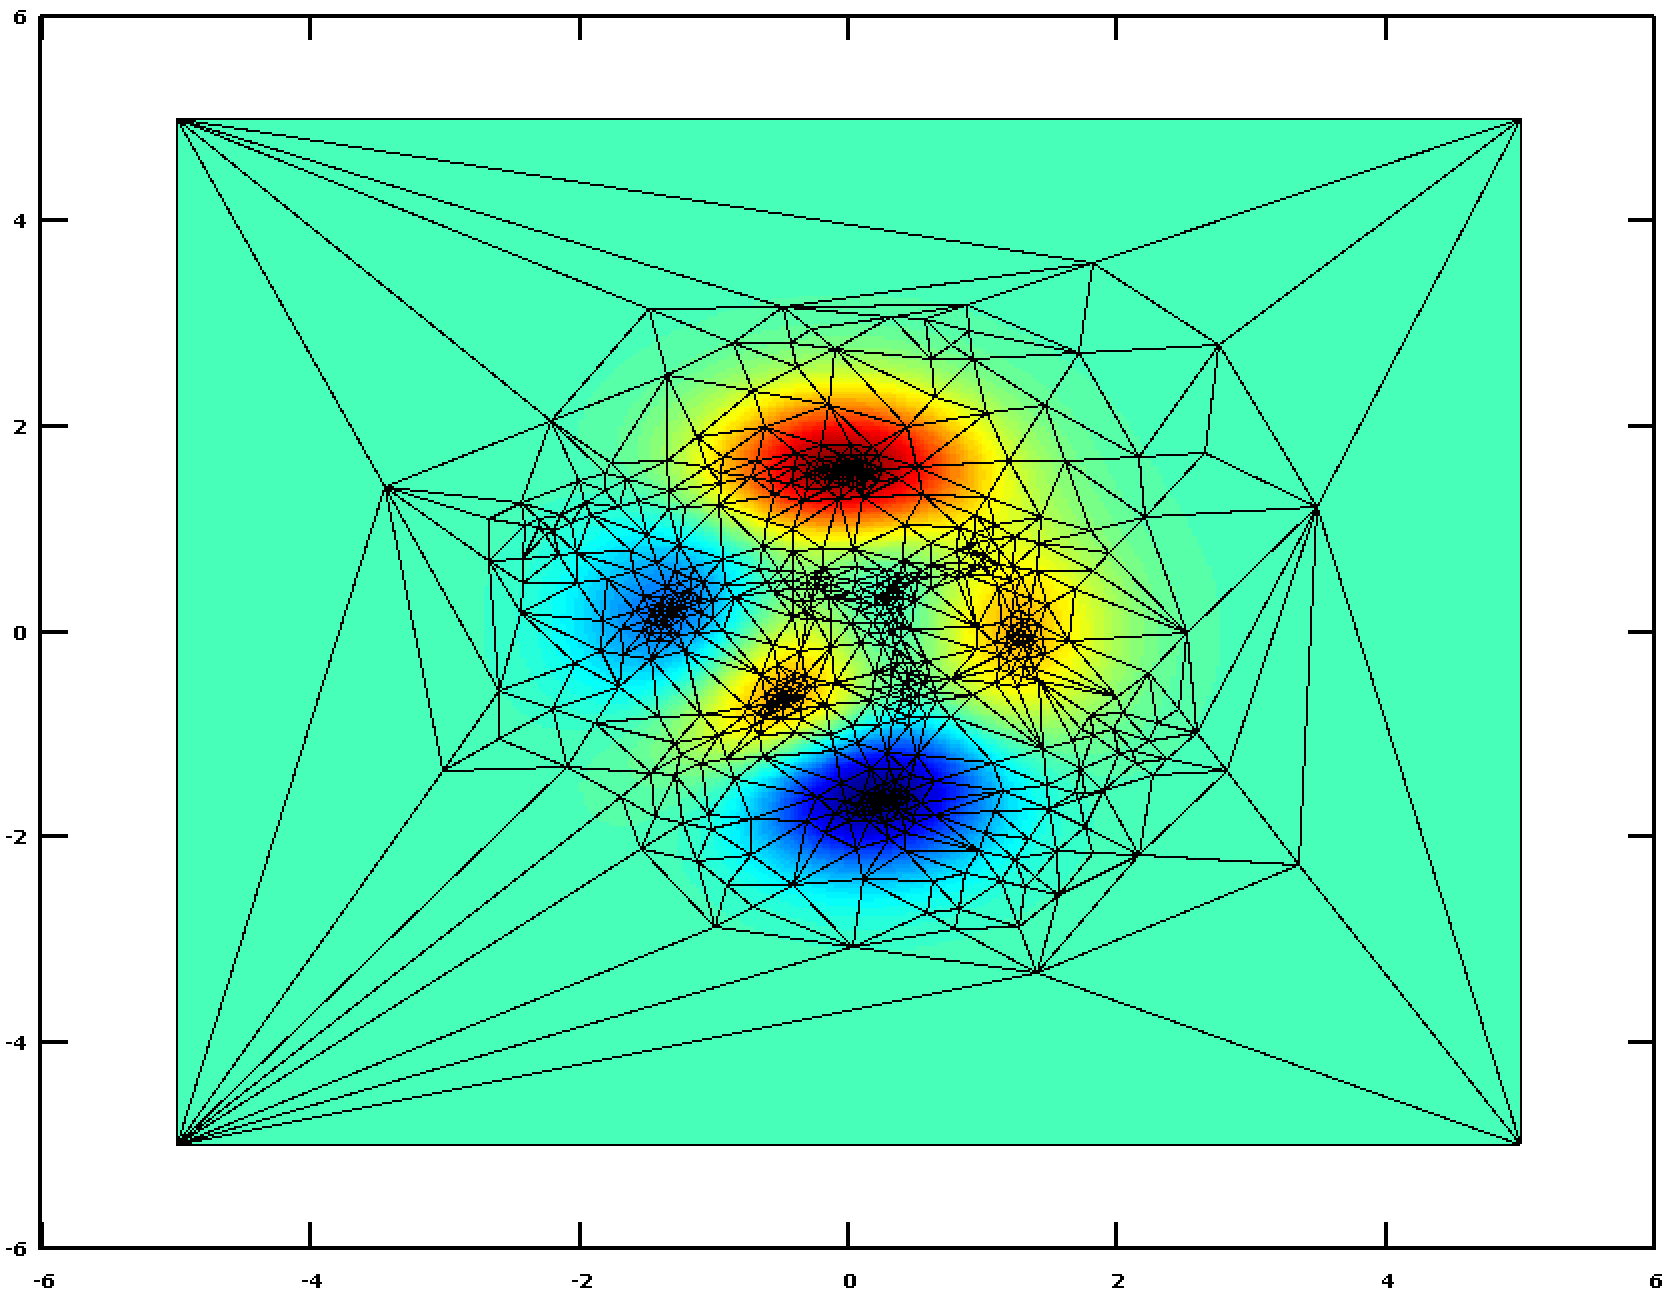
\includegraphics[width=50mm]{Figures/Reconnect025.png}}
  \end{center}
\end{figure}

In \ref{fig_ComboC} the marked difference in mesh quality and mesh
density caused by local reconnection can be seen. The addition of the
local reconnection enabled the quality of triangle to be improved every
step therefore allowed more nodes to be inserted. In this case, instead
of $92$ nodes being inserted (\ref{fig_ComboA}), $713$ nodes were
inserted. The surface area of the final mesh was $179.234$. This is a
representation deficit of $0.725\%$.
